
~\phantom{a}
	
\vskip 1cm


\noindent\makebox[.9\paperwidth]{
\noindent
\setlength\arrayrulewidth{4pt}
\begin{tabular}{p{.2\paperwidth}@{}!{\color{goldan-yellow}\vline width 1.5pt}p{.7\paperwidth}}
\hfill\raisebox{-3cm}{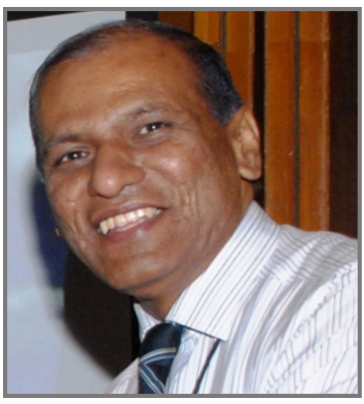
\includegraphics{src/Figures/Ramamurthy.jpg}~~}\newline\newline
\rule{.2\paperwidth}{.4pt}
 &
\bigskip
With the proliferation of data centres around the world, a need has arisen to efficiently store ‘Big data’ and at the same time protect the same from being lost due to failure of storage devices. Because of their huge volume, the data is often stored in multiple storage units in a distributed manner. In this scenario, to protect the data from being lost due to potential failure of storage devices, it has been the practice to replicate the data. The massive amount of data that is generated round the clock, the need for efficient storage and reliable retrieval has forced the industry to increasingly turn to erasure codes. Towards this direction, coding theorists have come up with two new classes of erasure codes known respectively as regenerating codes and locally recoverable codes. In their survey article titled “Erasure Coding for Big Data”, the authors provide their perspective overview of these two classes of codes.

\medskip
Moving on to an upcoming technical field that is bound to influence or change our lives is the field of Artificial Intelligence (AI). With this breakthrough technology, we have achieved success in directing machines to perform certain tasks using their intelligence. This all encompassing technology has found applications in the area of agriculture, astronomy, education, entertainment, sports, health care, automotive industry, etc.  In the article titled ‘AI Powered Society’, the author dwells on the influence of this technology. In doing so, he dwells on the way human society evolved over centuries from historical, philosophical and technological perspective.  He foresees our humanity to reassess the meaning of life, its place and significance in the universe, and above all its ability to survive in a world that includes its own creative creation – the super-intelligent, human-machine hybrid – the humanoid.

\medskip
In the information technology centric world that we live in, authentication is an important feature that every system or application software is expected to provide. In the article titled ‘An Overview of Authentication for Computer Communications’ the author describes commonly used password schemes along with standards. A brief overview of authentication used in cloud computing, Internet of Things (IOT) and Unique Identification Authority of India (UIDAI).

\medskip
Apart from the above, in our continuing series on experiential learning about the networking technology, the author describes the possible 11 states that a TCP connection can be in, and how the understanding of these states provide critical insight to diagnose the problem and resolve the same in the event of an abnormal behaviour. 

\vskip 3cm


\bigskip

\hfill  Dr. N Rama Murthy\hspace{2cm}\,

\hfill Editor\hspace{3cm}\,

\end{tabular}
}





